\documentclass[10pt]{beamer}

\usetheme{CambridgeUS}
\usepackage[english, russian]{babel}
\usepackage[utf8]{inputenc}
\usepackage{caption}
\usepackage{minted}
\usepackage{etoolbox}
\usepackage{multicol}
\AtBeginEnvironment{minted}{\singlespacing%
    \fontsize{10}{10}\selectfont}

\title[\href{https://goo.gl/NRgp8K}{https://goo.gl/NRgp8K} (Term 1)]{Введение в программирование}
\author[Гусев Илья, Булгаков Илья]{Гусев Илья, Булгаков Илья}
\institute[МФТИ] 
{Московский физико-технический институт\\*}
\date{Москва, 2018}
\subject{Computer Science}

\begin{document}

\begin{frame}
  \titlepage
\end{frame}

\begin{frame}{Содержание}
\tableofcontents
\end{frame}

\section{Введение}

\subsection{Структура курса}
\begin{frame}[fragile]{Структура курса}
\begin{enumerate}
\item Алгоритмы:
    \begin {itemize}
        \item 3 семестра
        \item Экзамены в 1 и 3
        \item 1 ак. час лекций в неделю
    \end {itemize}
\item C++:
    \begin {itemize}
        \item 2 семестра
        \item Экзамен во 2
        \item 1 ак. час лекций в неделю
    \end {itemize}
\item Практика
    \begin {itemize}
        \item 3 семестра,
        \item Во всех зачёты
        \item 2 ак. часа семинаров в неделю
    \end {itemize}
\end{enumerate}
Итого: 3 экзамена, 3 зачёта, 4 ак. часа в неделю на протяжении 3 семестров
\end{frame}

\subsection{Правила зачёта}
\begin{frame}[fragile]{Правила зачёта}{Оценки}
\begin{itemize}
\item 1 модуль - 25 балла
\item 2 модуль - 25 балла
\item 3 модуль - 25 балла
\item 4 модуль - 25 балла
\item 20 баллов за задачи и 5 баллов за ответ на контрольной
\item Сроки сдачи ограничены для каждого модуля
\item Критерий приёма задачи: Яндекс.Контест + review кода
\item Review кода = style + правильность алгоритма + функциональная декомпозиция
\end{itemize}
\end{frame}


\begin{frame}[fragile]{Правила зачёта}{Оценки}
\begin{itemize}
\item 0-39 баллов - 1 (неуд)
\item 40-49 баллов - 2 (неуд)
\item 50-56 баллов - 3 (удовл)
\item 57-65 баллов - 4 (удовл)
\item 66-71 баллов - 5 (хор)
\item 72-77 балла - 6 (хор)
\item 78-83 баллов - 7 (хор)
\item 84-88 баллов - 8 (отл)
\item 89-93 балла - 9 (отл)
\item 94-100 баллов - 10 (отл)
\end{itemize}
\end{frame}

\begin{frame}[fragile]{Правила зачёта}{Посещаемость, списывание, кодстайл}
\begin{itemize}
\item Про посещаемость: она напрямую не влияет на оценку
\item Про списывание: любое дублирование чужого кода штрафуется -5 и незачётом по задаче
\end{itemize}
\end{frame}

\begin{frame}[fragile]{Правила зачёта}{Кодстайл}
\begin{itemize}
\item Понятные названия переменных (однобуквенные только как счётчики в циклах или заданные в условии задачи)
\item Не должно быть утечек памяти
\item Грамтоная декомпозиция на функции. В main должен находиться ввод данных, вызов функции, которая решает задачу, вывод результата. Ввод/вывод производится только в main, решение - только в отдельном наборе функций
\item Переменные должны объявляться по месту использования (уже давно >= С99)
\item Глобальными переменными пользоваться нельзя
\item Остальное: \href{https://goo.gl/Ztu6td}{https://goo.gl/Ztu6td}
\end{itemize}
\end{frame}

\section{Про компьютеры}
\subsection{Транзисторы $\rightarrow$ Процессор}
\begin{frame}[fragile]{Транзисторы $\rightarrow$ Логические элементы}
\begin{itemize}
\item \href{http://www.cs.bu.edu/~best/courses/modules/Transistors2Gates/}{http://www.cs.bu.edu/$\sim$best/courses/modules/Transistors2Gates/}
\item \href{https://www.reddit.com/r/compsci/comments/209fqx/i_want_to_know_how_the_computer_works_from/}{Reddit topic: https://bit.ly/2CdBk3u}
\item \href{https://habr.com/post/338584/}{Реализация «Тетриса» в игре «Жизнь»: https://habr.com/post/338584/}
\end{itemize}
\end{frame}

\begin{frame}[fragile]{Транзисторы $\rightarrow$ Логические элементы}
\begin{multicols}{2}
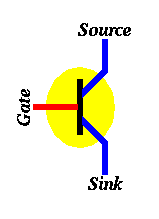
\includegraphics[width=3cm, height=4cm]{Term_1/Source/Pirctures/transistor-n.png}
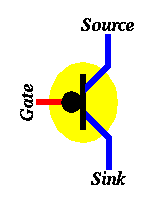
\includegraphics[width=3cm, height=4cm]{Term_1/Source/Pirctures/transistor-p.png}
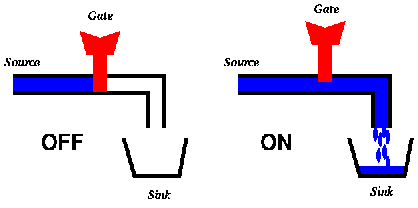
\includegraphics[width=6cm, height=4cm]{Term_1/Source/Pirctures/transistor-as-faucet.png}
\end{multicols}
\end{frame}

\begin{frame}[fragile]{Транзисторы $\rightarrow$ Логические элементы}{NOT}
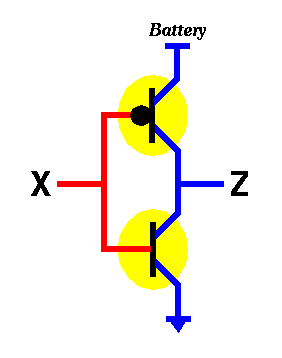
\includegraphics[width=6cm, height=6cm]{Term_1/Source/Pirctures/not-circuit.png}
\end{frame}

\begin{frame}[fragile]{Транзисторы $\rightarrow$ Логические элементы}{NAND}
\begin{multicols}{2}
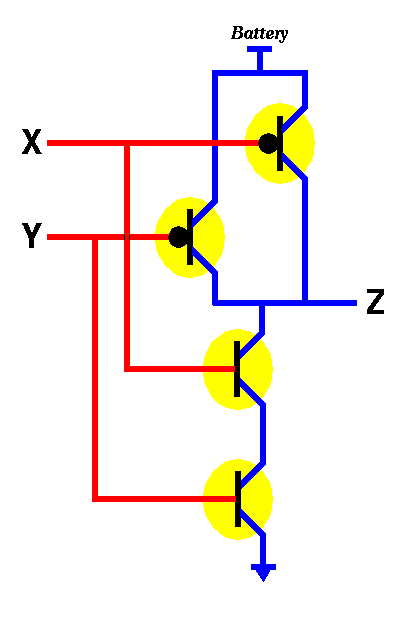
\includegraphics[width=5cm, height=7cm]{Term_1/Source/Pirctures/nand-circuit.png}
\vfill\eject
\begin{tabular}{ c|c|c } 
X &	Y & Z \\ 
  \hline
0 & 0 & 1\\
  \hline
0 & 1 & 1 \\
 \hline
1 & 0 & 1 \\
 \hline
1 & 1 & 0 \\
\end{tabular}
\end{multicols}
\end{frame}

\begin{frame}[fragile]{Транзисторы $\rightarrow$ Логические элементы}{NOR}
\begin{multicols}{2}
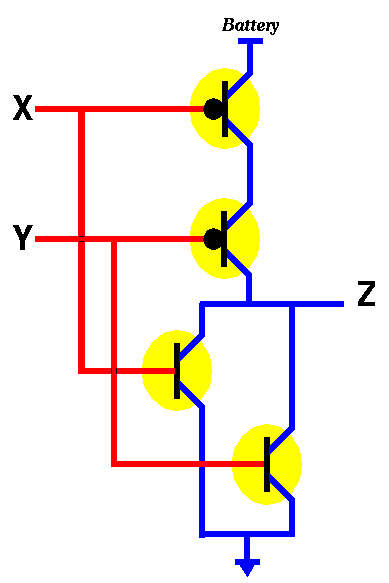
\includegraphics[width=5cm, height=7cm]{Term_1/Source/Pirctures/nor-circuit.png}
\vfill\eject
\begin{tabular}{ c|c|c } https://v2.overleaf.com/project/5849e163e473d1cf1e4b641d
X &	Y & Z \\ 
  \hline
0 & 0 & 1\\
  \hline
0 & 1 & 0 \\
 \hline
1 & 0 & 0 \\
 \hline
1 & 1 & 0 \\
\end{tabular}
\end{multicols}
\end{frame}

\begin{frame}[fragile]{Логические элементы $\rightarrow$ Сумматор}{AND, OR, XOR}
\begin{multicols}{2}
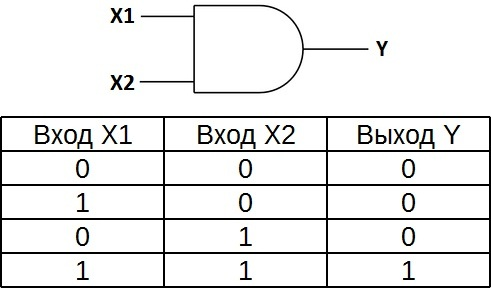
\includegraphics[width=4cm, height=3cm]{Term_1/Source/Pirctures/and.jpg}\\
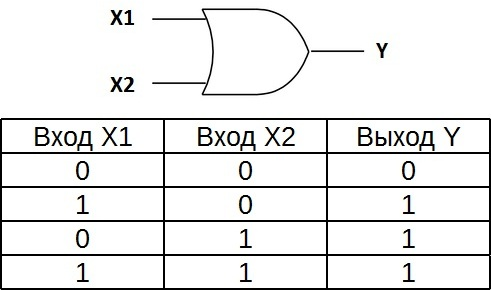
\includegraphics[width=4cm, height=3cm]{Term_1/Source/Pirctures/or.jpg}
\vfill\eject
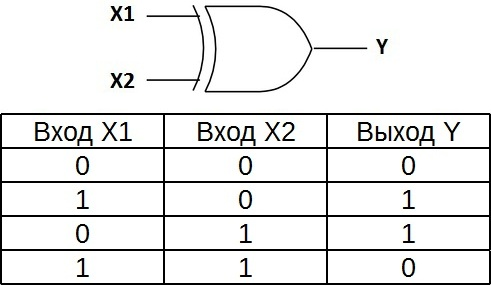
\includegraphics[width=4cm, height=3cm]{Term_1/Source/Pirctures/xor.jpg}
\end{multicols}
\end{frame}


\begin{frame}[fragile]{Логические элементы $\rightarrow$ Сумматор}{Half and full adder}
\begin{multicols}{2}
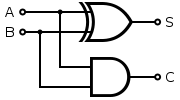
\includegraphics[width=4cm, height=3cm]{Term_1/Source/Pirctures/Half_Adder.png}
\vfill\eject
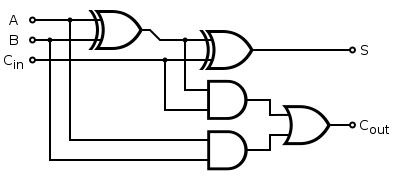
\includegraphics[width=4cm, height=3cm]{Term_1/Source/Pirctures/Full_Adder.png}
\end{multicols}
\end{frame}

\begin{frame}[fragile]{Логические элементы $\rightarrow$ Сумматор}{Линейный каскадный сумматор}
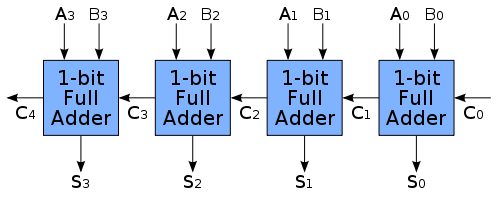
\includegraphics[width=8cm, height=3cm]{Term_1/Source/Pirctures/Ripple_carry_adder.png}
\end{frame}


\subsection{Память}
\begin{frame}[fragile]{Память}
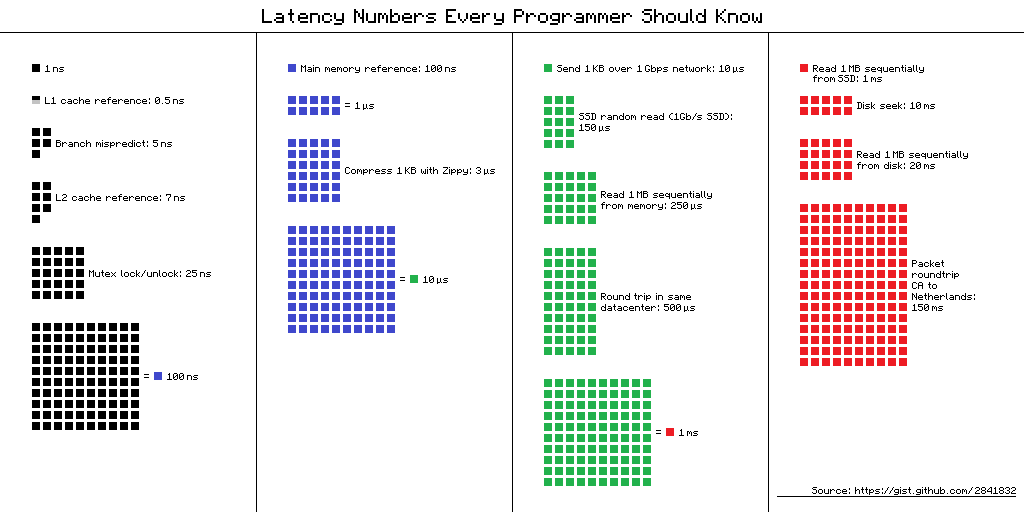
\includegraphics[width=12cm, height=7cm]{Term_1/Source/Pirctures/latency.png}
\end{frame}

\subsection{Архитектура фон Неймана}
\begin{frame}[fragile]{Архитектура фон Неймана}
\begin{itemize}
    \item Работа компьютера контролируется программой, состоящей из набора команд
    \item Принцип последовательного выполнения: после выполнения текущей команды IP (instruction pointer) автоматически указывает на следующую
    \item Принцип однородности: в памяти хранятся и данные, и команды
    \item Принцип адресуемости: память состоит из ячеек, каждая имеет уникальный «адрес»
    \item Использование двоичной системы счисления * (\href{https://habr.com/post/166679/}{https://habr.com/post/166679/})
\end{itemize}
\end{frame}

\begin{frame}[fragile]{Архитектура фон Неймана}
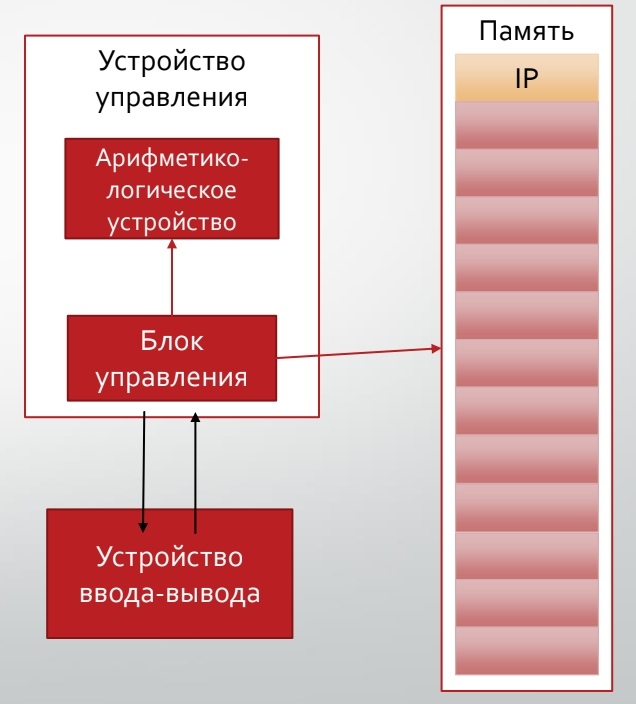
\includegraphics[width=7cm, height=7cm]{Term_1/Source/Pirctures/fon.jpg}
\end{frame}

\begin{frame}[fragile]{Архитектура фон Неймана}
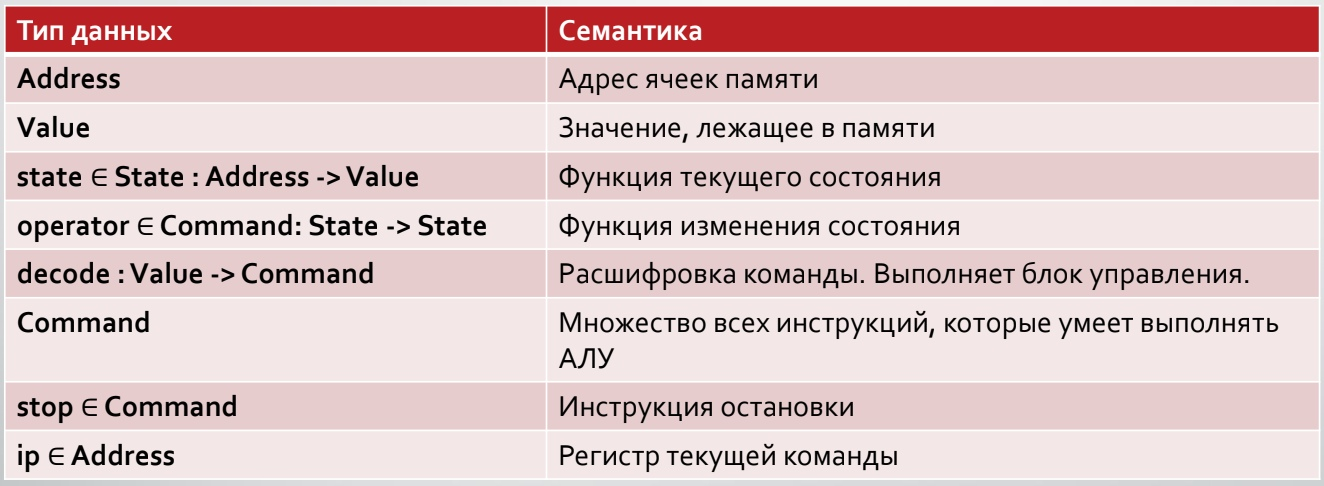
\includegraphics[width=12cm, height=5cm]{Term_1/Source/Pirctures/math-fon.jpg}\\
Принцип хранимой программы: $\forall c \in Command, \exists v \in Value : decode(v) = c $
Текущая операция: $operation = decode(state(state(ip)))$
\end{frame}


\begin{frame}[fragile]{Архитектура фон Неймана}{Пример}
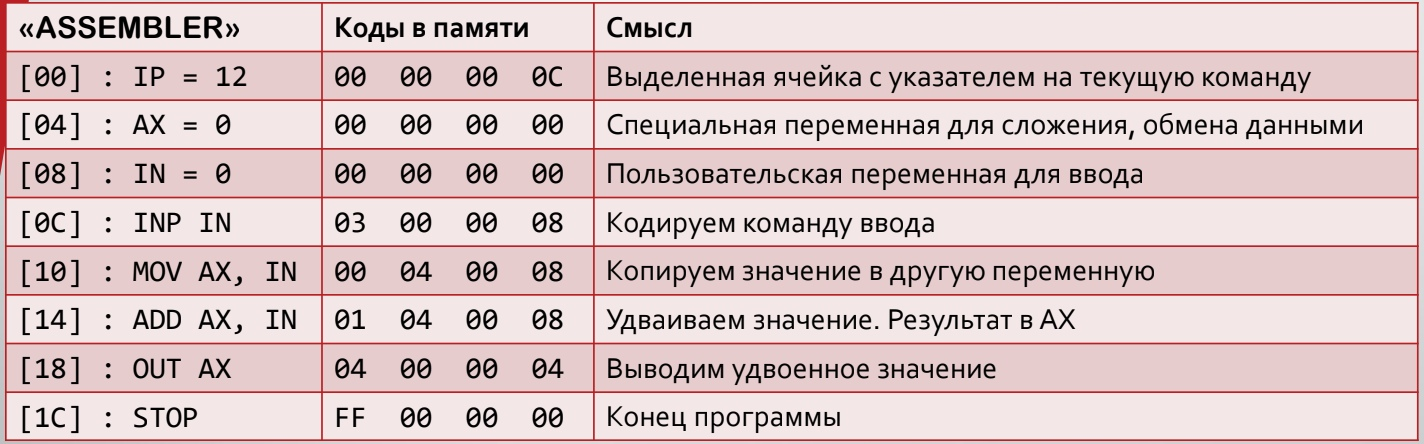
\includegraphics[width=12cm, height=4cm]{Term_1/Source/Pirctures/example.jpg}
\end{frame}

\begin{frame}[fragile]{Архитектура фон Неймана}{Пример}
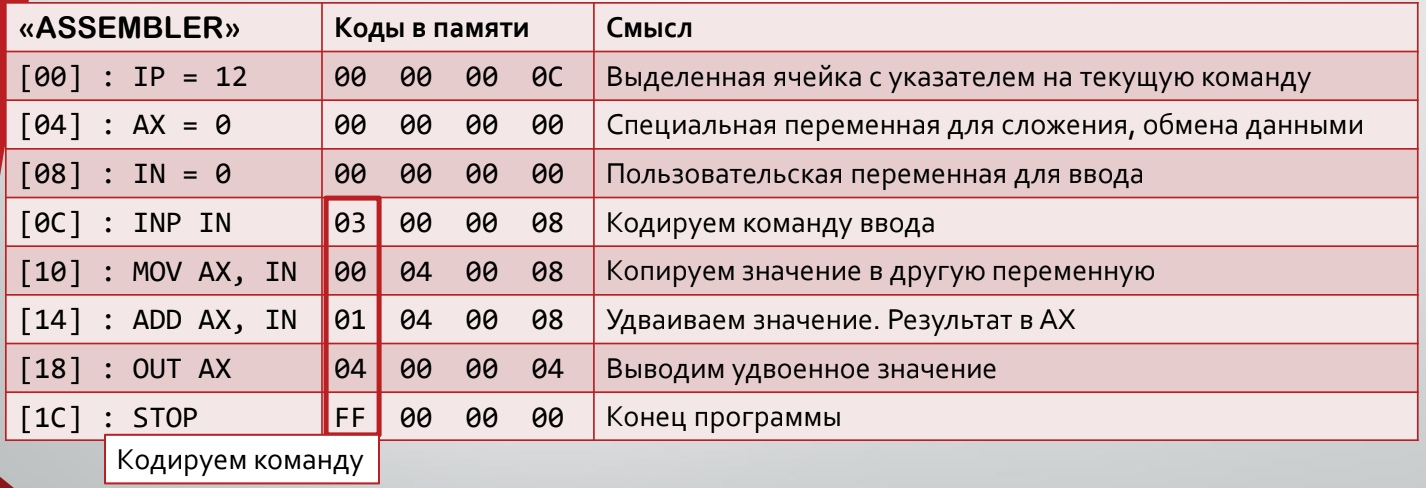
\includegraphics[width=12cm, height=4cm]{Term_1/Source/Pirctures/example1.jpg}
\end{frame}

\begin{frame}[fragile]{Архитектура фон Неймана}{Пример}
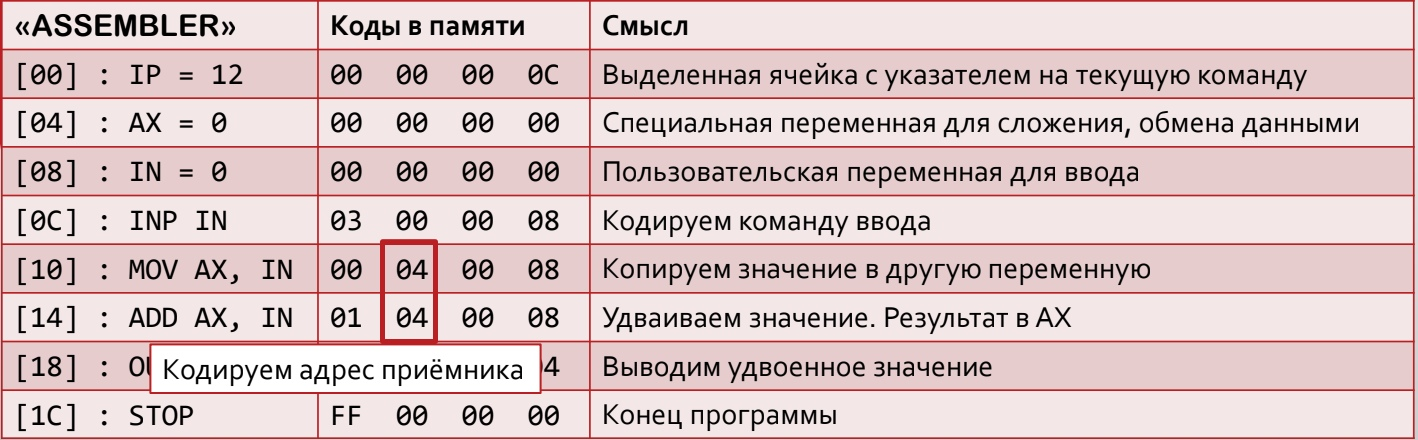
\includegraphics[width=12cm, height=4cm]{Term_1/Source/Pirctures/example2.jpg}
\end{frame}

\begin{frame}[fragile]{Архитектура фон Неймана}{Пример}
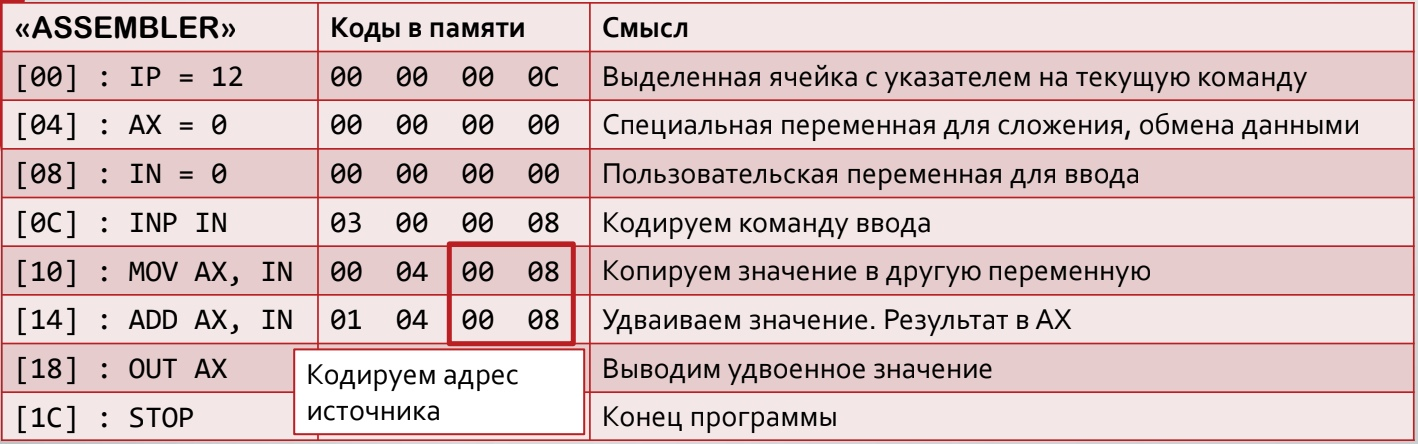
\includegraphics[width=12cm, height=4cm]{Term_1/Source/Pirctures/example3.jpg}
\end{frame}

\begin{frame}[fragile]{Архитектура фон Неймана}{Пример}
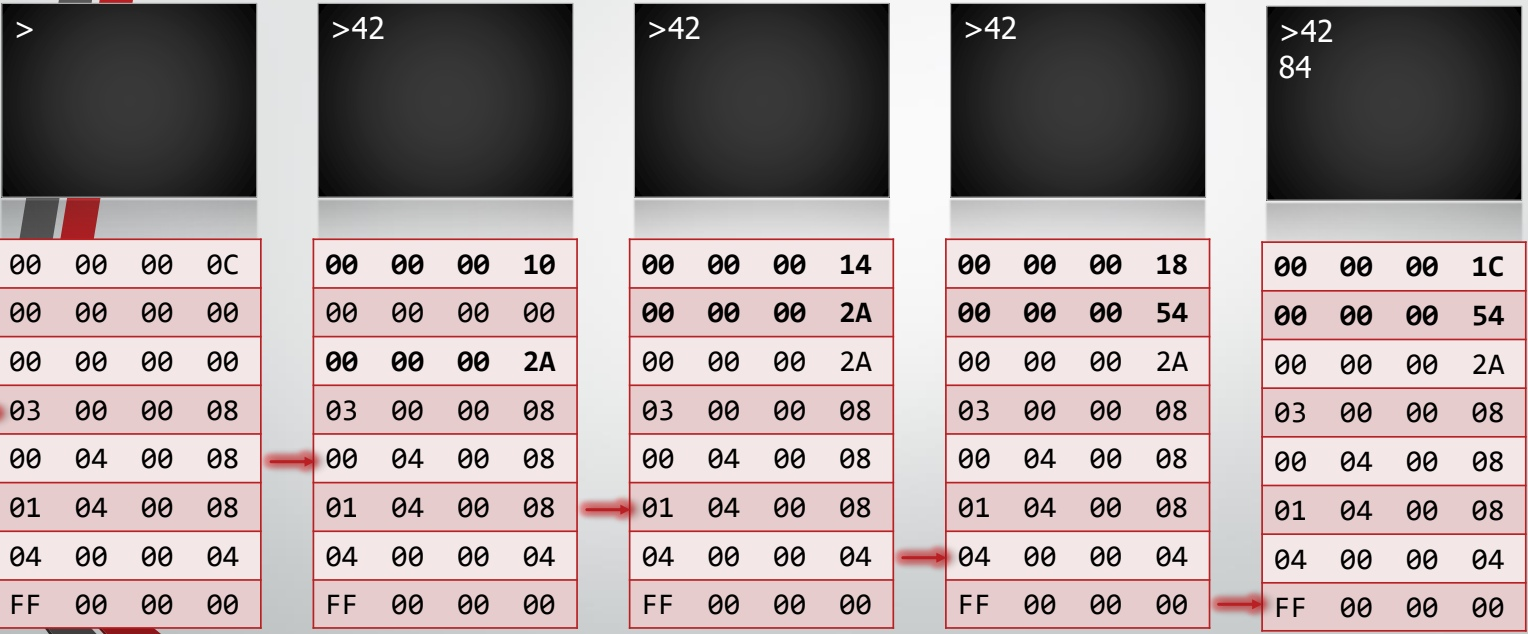
\includegraphics[width=12cm, height=5cm]{Term_1/Source/Pirctures/example-run.jpg}
\end{frame}

\section{Язык Си}
\subsection{Свойства языка}
\begin{frame}[fragile]{Свойства языка}
\begin{itemize}
    \item Компилируемый
    \item Процедурный
    \item Статически типизируемый
    \item Возможность модификации памяти через указатели
\end{itemize}
\end{frame}

\begin{frame}[fragile]{Компилируемость}
\begin{multicols}{2}
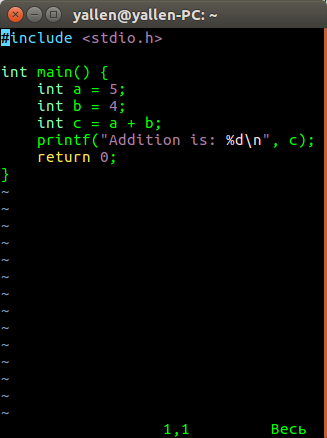
\includegraphics[width=5cm, height=7cm]{Term_1/Source/Pirctures/c-example.png}
\vfill\eject
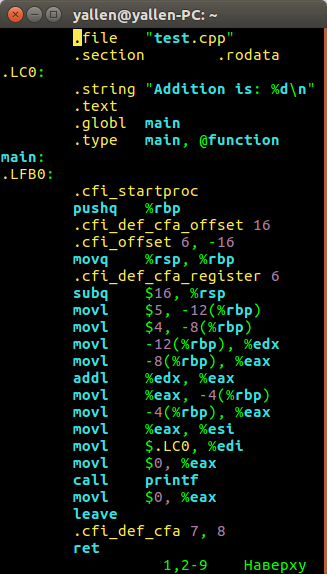
\includegraphics[width=4cm, height=7cm]{Term_1/Source/Pirctures/assembler-example.png}
\end{multicols}
\end{frame}

\begin{frame}[fragile]{Указатели}
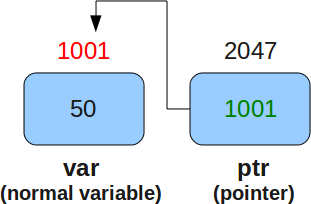
\includegraphics[width=8cm, height=5cm]{Term_1/Source/Pirctures/c-var-ptr.png}
\end{frame}

\appendix
\section<presentation>*{\appendixname}
\subsection<presentation>*{Useful links}

\begin{frame}[allowframebreaks]
  \frametitle<presentation>{Полезные ссылки}
    
  \begin{thebibliography}{10}
{
  \beamertemplatebookbibitems
  % Start with overview books.
  \bibitem{Kormen1}
  \texttt{Т.Кормен, Ч.Лейзерсон, Р.Ривест, К.Штайн - Алгоритмы. Построение и анализ. - 2013, djvu}
  \newblock \href{https://bit.ly/2wFzphU}{\texttt{https://bit.ly/2wFzphU}}
  
  \bibitem{Kormen2}
  \texttt{Т.Кормен, Ч.Лейзерсон, Р.Ривест, К.Штайн - Алгоритмы. Построение и анализ. - 2013, pdf}
  \newblock \href{https://bit.ly/2PpdqUc}{\texttt{https://bit.ly/2PpdqUc}}
  
  \bibitem{CKR}
  \texttt{Б.Керниган, Д.Ритчи - Язык программирования C - 2009, djvu}
  \newblock \href{https://bit.ly/2PwcVb8}{\texttt{https://bit.ly/2PwcVb8}}
  
  \bibitem{Lippman}
  \texttt{С.Липпман, Ж.Лажойе - Язык программирования C++. Базовый курс. - 2014, djvu}
  \newblock \href{https://bit.ly/2LQhk6z}{\texttt{https://bit.ly/2LQhk6z}}
  
  \bibitem{std}
  \texttt{Working Draft, Standard for Programming Language C++}
  \newblock \href{https://bit.ly/2PvGSIb}{\texttt{https://bit.ly/2PvGSIb}}
  
  \beamertemplatearticlebibitems
  
  \bibitem{wiki}
  \texttt{Викиконспекты}
  \newblock \href{http://neerc.ifmo.ru/wiki/}{\texttt{http://neerc.ifmo.ru/wiki/}}
  
  \bibitem{cppreference}
  \texttt{Справка по C++}
  \newblock \href{https://ru.cppreference.com/w/}{\texttt{https://ru.cppreference.com/w/}}
  
  \bibitem{superfaq}
  \texttt{C++ Super-FAQ}
  \newblock \href{https://isocpp.org/faq}{\texttt{https://isocpp.org/faq}}
   
  \bibitem{StackOverflow}
  \texttt{StackOverflow}
  \newblock \href{https://stackoverflow.com/}{\texttt{https://stackoverflow.com/}}
  
  \bibitem{Хабр}
  \texttt{Хабр}
  \newblock \href{https://habr.com/}{\texttt{https://habr.com/}}

}


  \end{thebibliography}
\end{frame}

\end{document}


